\documentclass[12pt]{article}
\hfuzz=5.002pt 

\usepackage{../advay} 
\usepackage{xcolor} 
\usepackage{graphicx}
\definecolor{ForestGreen}{rgb}{0.13, 0.55, 0.13} 
\definecolor{RubineRed}{rgb}{0.8, 0.0, 0.3} 
\definecolor{RoyalBlue}{rgb}{0.25, 0.41, 0.88}
\usepackage{graphicx}
\usepackage{biblatex}
\addbibresource{refs.bib}

\title{Meyers Lab Report \#2}
\author{Advay Vyas}
\date{\today}

\begin{document}
\maketitle

\tableofcontents


\section{Flu-Metrocast}
\subsection{Dashboard}
The dashboard has a scroller for the forecasts and the ability to select multiple forecasts. This forecast evaluation slider is quite neat, with the horizon at the end and how long the interval is. The evaluation tab also has a space to look at the various values and metrics for each forecast (as well as a heatmap). 

\section{Gradient boosting model}
I couldn't find the weighted interval score anywhere.
\subsection{Data preprocessing methods}
Removed COVID data to offset influenza and COVID mix-ups likely, added forecast targets. Used bags to ``bootstrap'' the data along with the gradient boosting. Used feature importance, how is that calculated? How is ``horizon'' the most important feature, isn't that we are predicting? Kept important features, scaled back to original, renamed, set up quantile. Made predictions using model.


\section{Alternative methods for prediction}
I just searched up some alternative methods and found the following:
\begin{itemize}
    \item Hierarchical forecast reconciliation
    \item Spatio-temporal GAMs (mixed-effects)
    \item Bayesian hierarchical spatio-temporal models
    \item Gaussian process regression
    \item Deep learning
\end{itemize}

\section{R package creation}
I'm taking notes on ``R Packages (2e)'' by Hadley Wickham and Jennifer Bryan.

\subsection{The Whole Game}
Devtools package is useful for package development. Devtools automatically creates a \verb|.gitignore| and likely has an implementation for Git usage outside of beginning in a Git repo (actually recommended to not do that). The command to use Git (in any R project) is \verb|use_git()|. We save function definitions in the \verb|function\_name.R| file in the folder. The \verb|check()| function is the ``gold standard'' of checking R packages completely work.

Editing the DESCRIPTION file is important, we can do stuff like declaring an author, titling the package, version number, etc. Also important is declaring a license (MIT license will probably do just fine). Additionally, we need to add documentation to our functions and code so that users know how to use them in the future. We use \textit{Code $\rightarrow$ Insert roxygen skeleton} to create our documentation boilerplate and then fill it out from there, then using \verb|document()| to update the documentation. Help file can now be accessed like any other native function in R, with \,?function\_name. We can now \verb|install()| the package into our library. 

To write unit tests for our code, we use the \verb|use_testthat()| funciton that starts the unit testing creation process. You can open a test file with \verb|use_test()|. To use another package in your code (even functions that are often already in the default like \verb|stats::median()| or \verb|utils::head()|), you must use the \verb|use_package()| command. 

To use GitHub for R package development, it's recommended to start early with \verb|use_github()|. Also, \verb|use_readme_rmd()| initializes the file for easy editing and \verb|build_readme()| renders the file. Lastly, the book recommends us to commit often, \verb|check()| often, and \verb|install()| often.

\begin{figure}
    \centering
    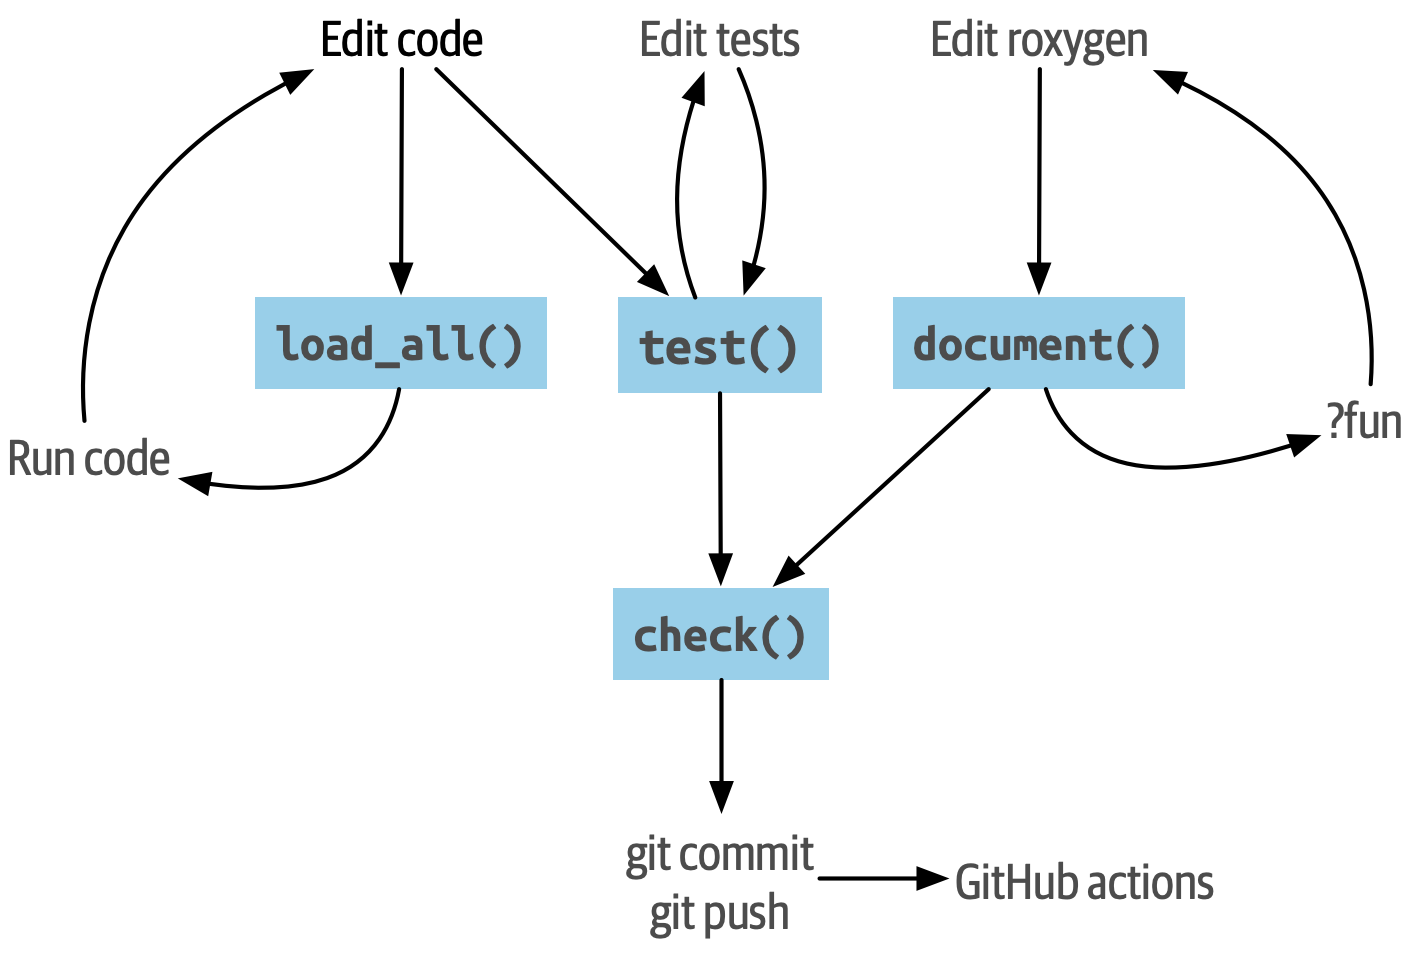
\includegraphics[width=0.8\linewidth]{workflow.png}
    \caption{A picture of the package workflow from the book}
\end{figure}

\pagebreak

A list of useful functions:
\begin{itemize}
    \item \verb|create_package()|
    \item \verb|use_git()|
    \item \verb|use_mit_license()|
    \item \verb|use_testthat()|
    \item \verb|use_github()|
    \item \verb|use_readme_rmd()|
    \item \verb|use_r()|
    \item \verb|use_test()|
    \item \verb|use_package()|
    \item \verb|load_all()|
    \item \verb|document()|
    \item \verb|test()|
    \item \verb|check()|
\end{itemize}


\end{document}